\documentclass[11pt]{article}
\usepackage{acl2014}
\usepackage{times}
\usepackage{url}
\usepackage{latexsym}
\usepackage{hyperref}
\usepackage{graphicx}

\title{Name of your project}

\author{Sergio Kazatzidis \\
    {\tt sergio@example.com} \\
    Kamiel Fokkink \\
    {\tt kamielfokkink@gmail.com} \\\And
    Baran İşcanlı \\
    {\tt barantevitol@gmail.com} \\
    Tomas Kehus \\
    {\tt tekehus@gmail.com}}

\date{}

\begin{document}
\maketitle
\begin{abstract}
    This is where we write our abstract
\end{abstract}

\noindent

\section{Introduction}

\section{Dataset}
The dataset that we used for the training of our model was Amazon review data, which was retrieved from \href{http://jmcauley.ucsd.edu/data/amazon/}{here}. This database contains review information about numerous kinds of products, ranging from groceries to clothes to video games. But reviews about for example kitchen appliances would say more about the quality of the product, and not about a consumers individual tastes. The most suitable kinds of products to train a recommender system on are those of which the review reflects the particular persons interests and tastes. Therefore, we chose to use the datasets of Kindle books, video games, and digital music. The database offers two options for the dataset: all aggregated reviews, or a filtered dataset to only include reviewers that rated 5 or more products. We chose the second option, because it reduces the cost of training, and it is more relevant to have several datapoints per user, so as to have more information for good recommendations. \\

\subsection{Splitting the data}
The sizes of the datasets are: 31MB and 64k lines for the music, 110MB and 231k lines for the video games, and 266MB and 982k lines for the books. For each review, there are several features that we can include. Some are necessary for our analysis, such as the reviewer ID, product ID, and the review score. Many features are also less relevant for our purposes, but can be included if needed, such as the review time or a review text. A printout sample of the data can be seen in figure 1. \\
\begin{figure}
    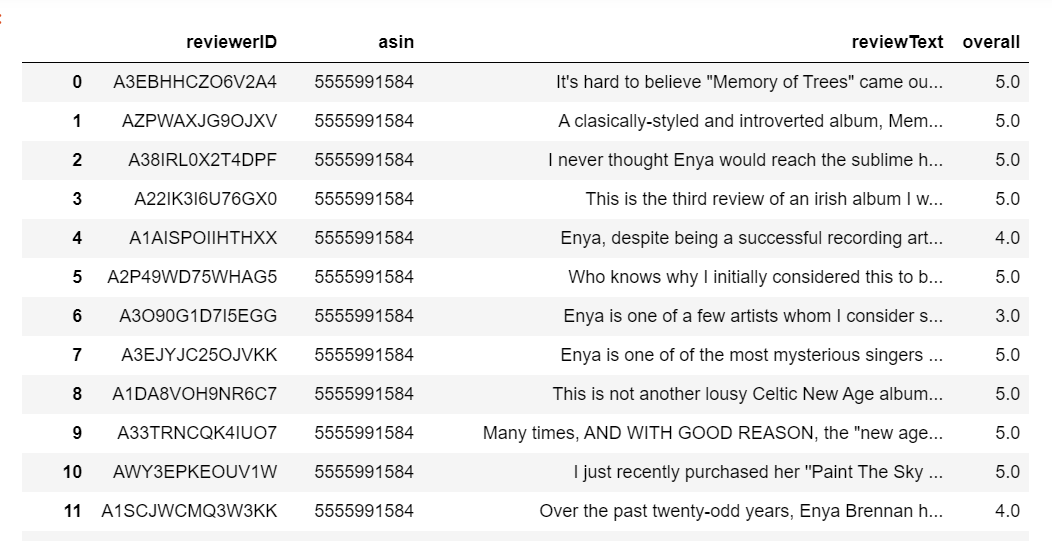
\includegraphics[width=10cm]{Pandas_df_example.png}
    \caption{Pandas dataframe of the data}
\end{figure}

For testing purposes, we want to split our data into a training and a testing set. This is not just a simple randomized split of the datapoints. For the evaluation of our recommender system, we need to split our user base, taking out 10\% of all users and putting them in a test set. Our test set will therefore consist of completely new users who have not been used for the training of our model. By looking at a few of those new user's preferences, the model can then recommend them new items to buy. We will be able to compare these recommendations to our expected recommendations, to evaluate our model.

\end{document}
